\documentclass[a4paper,12pt]{extarticle}
\usepackage{geometry}
\usepackage[T1]{fontenc}
\usepackage[utf8]{inputenc}
\usepackage[english,russian]{babel}
\usepackage{amsmath}
\usepackage{amsthm}
\usepackage{amssymb}
\usepackage{fancyhdr}
\usepackage{setspace}
\usepackage{graphicx}
\usepackage{colortbl}
\usepackage{tikz}
\usepackage{pgf}
\usepackage{subcaption}
\usepackage{listings}
\usepackage{indentfirst}
\usepackage[
backend=biber,
style=numeric,
maxbibnames=99
]{biblatex}
\addbibresource{refs.bib}
\usepackage[colorlinks,citecolor=blue,linkcolor=blue,bookmarks=false,hypertexnames=true, urlcolor=blue]{hyperref} 
\usepackage{indentfirst}
\usepackage{mathtools}
\usepackage{booktabs}
\usepackage[flushleft]{threeparttable}
\usepackage{tablefootnote}

\usepackage{chngcntr} % нумерация графиков и таблиц по секциям
\counterwithin{table}{section}
\counterwithin{figure}{section}

\graphicspath{{graphics/}}%путь к рисункам

\makeatletter
% \renewcommand{\@biblabel}[1]{#1.} % Заменяем библиографию с квадратных скобок на точку:
\makeatother

\geometry{left=2.5cm}% левое поле
\geometry{right=1.0cm}% правое поле
\geometry{top=2.0cm}% верхнее поле
\geometry{bottom=2.0cm}% нижнее поле
\setlength{\parindent}{1.25cm}
\renewcommand{\baselinestretch}{1.5} % междустрочный интервал


\newcommand{\bibref}[3]{\hyperlink{#1}{#2 (#3)}} % biblabel, authors, year
\addto\captionsrussian{\def\refname{Список литературы (или источников)}} 

\renewcommand{\theenumi}{\arabic{enumi}}% Меняем везде перечисления на цифра.цифра
\renewcommand{\labelenumi}{\arabic{enumi}}% Меняем везде перечисления на цифра.цифра
\renewcommand{\theenumii}{.\arabic{enumii}}% Меняем везде перечисления на цифра.цифра
\renewcommand{\labelenumii}{\arabic{enumi}.\arabic{enumii}.}% Меняем везде перечисления на цифра.цифра
\renewcommand{\theenumiii}{.\arabic{enumiii}}% Меняем везде перечисления на цифра.цифра
\renewcommand{\labelenumiii}{\arabic{enumi}.\arabic{enumii}.\arabic{enumiii}.}% Меняем везде перечисления на цифра.цифра

\begin{document}
\begin{titlepage}
    \newpage
    
    {\setstretch{1.0}
    \begin{center}
    ПРАВИТЕЛЬСТВО РОССИЙСКОЙ ФЕДЕРАЦИИ\\
    ФГАОУ ВО НАЦИОНАЛЬНЫЙ ИССЛЕДОВАТЕЛЬСКИЙ УНИВЕРСИТЕТ\\
    «ВЫСШАЯ ШКОЛА ЭКОНОМИКИ»
    \\
    \bigskip
    Факультет компьютерных наук\\
    Образовательная программа «Прикладная математика и информатика»
    \end{center}
    }
    
    \vspace{2em}
    УДК 004.421.2 % УДК нужно указывать только для исследовательсвого проекта - удалите эту строку для программного проекта
    \vspace{4em}
    
    \begin{center}
    %Выберите какой у вас проект
    {\bf Отчет об исследовательском проекте на тему:}\\
    %{\bf Отчет о командном исследовательском проекте на тему:}\\
    %{\bf Отчет о программном проекте на тему:}\\
    %{\bf Отчет о командном программном проекте на тему:}\\
    {\bf Гиперэвристика алгоритмов роевого интеллекта}\\
    % строчка ниже нужна только при сдача плана КР, при финальной сдаче закомментируйте ее
    (промежуточный, этап 1)
    \end{center}
    
    \vspace{2em}
    
    {\bf Выполнил студент: \vspace{2mm}}
    %{\bf Выполнили студенты: \vspace{2mm}}
    
    {\setstretch{1.1}
    \begin{tabular}{l@{\hskip 1.5cm}l}
    группы \#БПМИ236, 2 курса & Коростелев Данил Александрович \\
    %группы \#БПМИ172, 3 курса & Петров Андрей Алексеевич \\
    %группы \#БПМИ173, 3 курса & Иванов Андрей Алексеевич 
    \end{tabular}}
    
    % Обычно у вас есть один научный руководитель, и это человек, с которым вы работаете над проектом. Иногда по формальным причинам у вас будет руководитель (штатный сотрудник Вышки) и соруководитель (тот, с кем вы работаете), — об этом вам сообщит учебный офис (в случае с ВКР) или ЦППРиП (в случае с курсовым проектом). Также, если кто-то дополнительно вам помогал, то его можно указать как консультанта. 
    
    %ваш официальный научник (из ВШЭ)
    \vspace{1em}
    {\bf Принял руководитель проекта: \vspace{2mm}}
    
    {\setstretch{1.1}
    \begin{tabular}{l}
    Родригес Залепинос Рамон Антонио\\
    Научный сотрудник\\
    Факультет компьютерных наук НИУ ВШЭ 
    \end{tabular}}
    
    % со-руководитель (если есть)
    %\vspace{1em}
    %{\bf Соруководитель: \vspace{2mm}}%это ваш официальный научник
    
    %{\setstretch{1.1}
    %\begin{tabular}{l}
    %Петрова Надежда Александровна\\
    %Инженер-исследователь\\
    %ОАО Компания "Нейросети и деревья" 
    %\end{tabular}}
    
    % консультант (если есть)
    %\vspace{1em}
    %{\bf Консультант: \vspace{2mm}}%это ваш официальный научник
    
    %{\setstretch{1.1}
    %\begin{tabular}{l}
    %Иванова Надежда Александровна\\
    %Инженер-исследователь\\
    %ОАО Компания "Нейросети и деревья" 
    %\end{tabular}}
    
    \vspace{\fill}
    
    \begin{center}
    Москва 2024
    \end{center}
    
    \end{titlepage}% это титульный лист - выберите подходящий вам из имеющихся в проекте вариантов (kr - курсовая работа у 3 курса, vkr - выпускная квалификационная работа у 4 курса)
\newpage
\setcounter{page}{2}

{
	\hypersetup{linkcolor=black}
	\tableofcontents
}

\newpage

\newpage
\section*{Аннотация}   % this is how to use russian
Курсовая работа посвящена исследованию и реализации новой гиперэвристики алгоритмов роевого интллекта World Hyper-Heuristic (WHH). В рамках работы проводится анализ существующих алгоритмов роевого интеллекта для дискретных или непрерывных задач оптимизации, таких как алгоритм муравьиной колонии (ACO), оптимизация роем частиц (PSO) и других, с целью выявления их сильных и слабых сторон. Основное внимание уделяется гиперэвристикам — методам, которые позволяют автоматически комбинировать и адаптировать низкоуровневые эвристики для решения сложных оптимизационных задач.

Цель работы заключается в проверке нового алгоритма WHH, на оптимизационных задачах в многомерных пространствах и предложении модификаций, направленных на улучшение качества и скорости сходимости алгоритма. В ходе исследования планируется изучить предложенный алгоритм и провести его тестирование на стандартных наборах задач оптимизации. Результаты работы будут сравниваться с существующими алгоритмами роевого интеллекта для оценки их производительности и качества решений.

Ключевые аспекты работы включают: изучение теоретических основ роевого интеллекта и гиперэвристик, исследование реализации архитектуры нового алгоритма, предложение модификаций и оптимизаций, и экспериментальное исследование. Практическая значимость работы заключается в возможности применения разработанного алгоритма для решения задач оптимизации в различных областях, таких как машинное обучение, управление ресурсами, планирование и другие.

\addcontentsline{toc}{section}{Аннотация}

\section*{Ключевые слова}
Обучение с подкреплением, NP-hard, Роевой интеллект
\pagebreak

\section{Введение}	

Всю историю человечество сталкивается с необходимостью решения различных задач как можно быстрее и экономнее в контексте ресурсов, что неизбежно привело к появлению алгоритмов различной сложности, решающих эти задачи. Многие задачи имеют решения среди алгоритмов полиномиальной сложности, например сортировка массива чисел. Такие алгоритмы в худшем случае требуют веремя пропорциональное $C \times n^k$, где $n$ - размер входных данных, а $C$ и $k$ - константы.  

Однако не все задачи могут быть решены при помощи алгоритма полиномиальной сложности (споры об этом до сих пор продолжаются, однако пока что существование таких алгоритмов для всех задач не доказано), к таким задачам относится например проблема комивояжера - оптимизационная задача поиска циклического маршрута с наименьшей стоимостью через все узлы взвешенного графа. Проблема коммивояжера относится к NP-сложным.

Современные задачи оптимизации, возникающие в различных областях науки и техники, зачастую характеризуются высокой сложностью, многомерностью и наличием ограничений. Традиционные методы оптимизации зачастую оказываются недостаточно эффективными для решения таких задач, что стимулирует развитие новых подходов. Одним из таких направлений являются алгоритмы роевого интеллекта, которые имитируют коллективное поведение природных систем, таких как стаи птиц, колонии муравьев или косяки рыб~\cite{trivedi_varshney}. Эти алгоритмы позволяют с приемлимой скоростью находить субоптимальные решения.

Такие алгоритмы называются метаэвристиками, они начинают с случайного решения и постепенно улучшают его при помощи исследования, иначе говоря, поиска решений, не являющихся близкими к текущему, или эксплуатации, то есть поиска решений среди близких к текущему. Очень важно чтобы алгоритм соблюдал баланс между этими подходами.

Согласно No Free Lunch Theory~\cite{nofreelunch} каждый из этих алгоритмов будет хорош лишь для определенного подмножества проблем и найти универсальный алгоритм не получится. Тут на помощь приходят Гиперэвристики~\cite{burke_etal_2019} - комбинации метаэвристик. Такие алгоритмы переключаются между различными метаэвристиками и позволяют свести задачу к выбору подходящего решения вместо его поиска, а также позволяют лучше контролировать соотношение исследования и эксплуатации.

В 2024 году ученые из университетов Ирана и США предложили свой алгоритм, основанный на гиперэвристике алгоритмов роевого интеллекта, названный World Hyper-Heuristic~\cite{WHH}. Приведенные в статье данные демонстрируют значительное превосходство WHH над самыми известными метаэвристиками, что не могло не привлечь внимание к теме. В своей курсовой работе я постраюсь воспроизвести результаты полученные в статье и предложу возможные улучшения и оптимизации.

\section{Эвристики, Метаэвристики, Гиперэвристики}

Для понимания контекста критически важно разобраться в терминологии, а именно в том, что такое и чем ращличаются эвристики, метаэвристики и гиперэвристики.

Эвристика (эвристический алгоритм) - алгоритм, основывающийся на практике, не являющийся гарантированно точным или оптимальным, но достаточный для решения (ускорения решения) поставленной задачи\footnote{Согласно Википедии: \url{https://en.wikipedia.org/wiki/Heuristic}}

Самое частое применение эвристик - неалгоритмическая оптимизация алгоритма. Эвристикой могут быть такие простые правила как "выбирать всегда первый элемент" или "всегда решать сначала более сложные задачи".

Метаэвристика гораздо более сложное понятие. Это высокоуровневые алгоритмы, которые направляют процесс поиска решений для оптимизационных задач. Они разработаны для работы с широким спектром проблем и часто вдохновлены природными процессами. В отличие от эвристик, которые обычно специфичны для задачи, метаэвристики универсальны и могут адаптироваться к различным сценариям.

Особое место занимают метаэвристики роевого интеллекта, которые имитируют коллективное поведение децентрализованных систем в природе, таких как стаи птиц, колонии муравьёв или косяки рыб. Примеры:
\begin{itemize}
    \item Оптимизацию роем частиц (PSO) — моделирует движение частиц в пространстве поиска, вдохновлённое поведением стаи.
    \item Оптимизацию муравьиной колонией~\cite{ACO} (ACO) — основана на том, как муравьи находят кратчайший путь, используя феромоны.
    \item Алгоритм отжига~\cite{SA} (SA) — алгоритм вдохновлен процессом отжига при обработке металла.
\end{itemize}
Эти алгоритмы работают, поддерживая популяцию потенциальных решений и улучшая их итеративно через процессы, напоминающие естественное поведение, такие как движение, коммуникация и адаптация.

К сожалению метаэвристики позволяют найти только субоптимальные решения задачи, однако этого достаточно для большинства реальных задач, поэтому метаэвристики получили большое распространение в промышленной разработке. 

Ключевыми понятиями в метаэвристиках является исследование (exploration) и эксплуатация (exploitation) первое отвечает за поиск новых решений, не похожих на текущее найденное решение, что позволяет таким алгоритмам не застревать в локальном оптимуме. Эксплуатация в свою очередь позволяет алгоритму улучшать найденное хорошее решение. Очень важно, чтобы алгоритм соблюдал баланс между этими двумя процессами.

Гиперэвристики - следующий уровень абстракции. Эти методы работают над выбором, комбинацией различных метаэвристик для эффективного решения конкретной задачи. Гиперэвристики ищут в пространстве метаэвристик, а не в пространстве решений, что сильно отличает их от метаэвристик.

В контексте алгоритмов роевого интеллекта гиперэвристики могут быть использованы для определения, какой метаэвристический подход лучше всего подходит для данной задачи. Гиперэвристики могут быть как очень простыми, как запуск последовательности эвристик и метаэвристик~\cite{Thompson}, так и сложными, например с применением обучения с подкреплением, как гиперэвристика, которую я буду рассматривать далее.

\section{Обзор литературы}

Основным источником для моей работы служит статья, которую я как раз и исследую, это статья~\cite{WHH} представленная в 2024 году иранскими и американскими учеными, описывает новый алгоритм поиска субоптимальных решений, который базируется на гиперэвристическом подходе к оптимизации, но при этом сочетает в себе множество других популярных приемов.

Так например авторы в своем алгоритме используют адаптивный подход, основанный на "обучении с подкреплением", эта сфера очень активно развивается, как и все сообщество программистов как-либо связанных с машинным обучением. 

Недавние тенденции в области гиперэвристик, описанные в обзоре Докероглу и др.~\cite{taxonmy} из 2023 года, подчеркивают интеграцию машинного обучения и оптимизации с несколькими целями, расширяя их применимость. Таксономия включает выборочные гиперэвристики, низкоуровневые эвристики и параллельные подходы, отражая зрелость области за последние 20 лет. Эти разработки предполагают, что рамки обучения с подкреплением WHH могут быть расширены для сценариев с несколькими целями, решая сложные реальные задачи, такие как устойчивое преобразование, как отмечено в недавних сессиях IEEE CEC. 

\section{World Hyper-Heuristic (WHH)}

В этой главе я подробно опишу принцип работы исследуемого алгоритма, а также приложу иллюстрации приведенные авторами, также опишу структуру кода реализации алгоритма, приведенную авторами статьи.

WHH или мировой алгоритм использует технику обучения с подкреплением для оптимизации выбора алгоритма на каждом шаге, метаэвристики из которых выбирает WHH определяются разработчиком, о том какие алгоритмы выбрали авторы статьи и о своих экспериментов я расскажу в секции экспериментов. 

Оптимизация обучением с подкреплением должна помочь избежать ситуации, когда гиперэвристика зацикливается на одной метаэвристике.

Оптимизация состоит из двух шагов - вознаграждения и селекции.

На первом шаге алгоритм делает обоснованное предположение о том, как каждый алгоритм поведет себя в дальнейшем, а затем на этапе селекции WHH выбирает лучший алгоритм о том, как происходит награждение и выбор расскажу поподробнее далее.

Приложу также иллюстрацию из оригинальной статьи которая должа дать базовое понимание устройства WHH~\ref{fig:basic_whh}. 

В целом работу алгоритма можно разделить на 3 фазы, который проиллюстрированы на рисунке~\ref{fig:complex_whh}: 

\begin{enumerate}
	\item Фаза инициализации, или первая итерация
	\item Фаза "обучения"
	\item Фаза вычисления функции потерь
\end{enumerate}

Во время фазы инициализации генерируется начальная популяция решений, а затем метаэвристики получают свои вознаграждения в зависимости от результатов полученных на этой популяции, на следующей итерации выбор алгоритма будет основан на результатах полученных на этой фазе.

Фаза обучения это основная фаза, выбора следующей метаэвристики, подробное описание этой фазы есть в разделе селекции.

В фазу вычисления, выбранный на предыдущем этапе алгоритм запускается на текущей популяции и вычисляются функции потерь, затем, если не превышено максимальное число итераций, алгоритм возвращается к фазе "обучения".

\begin{figure}
	\centering
	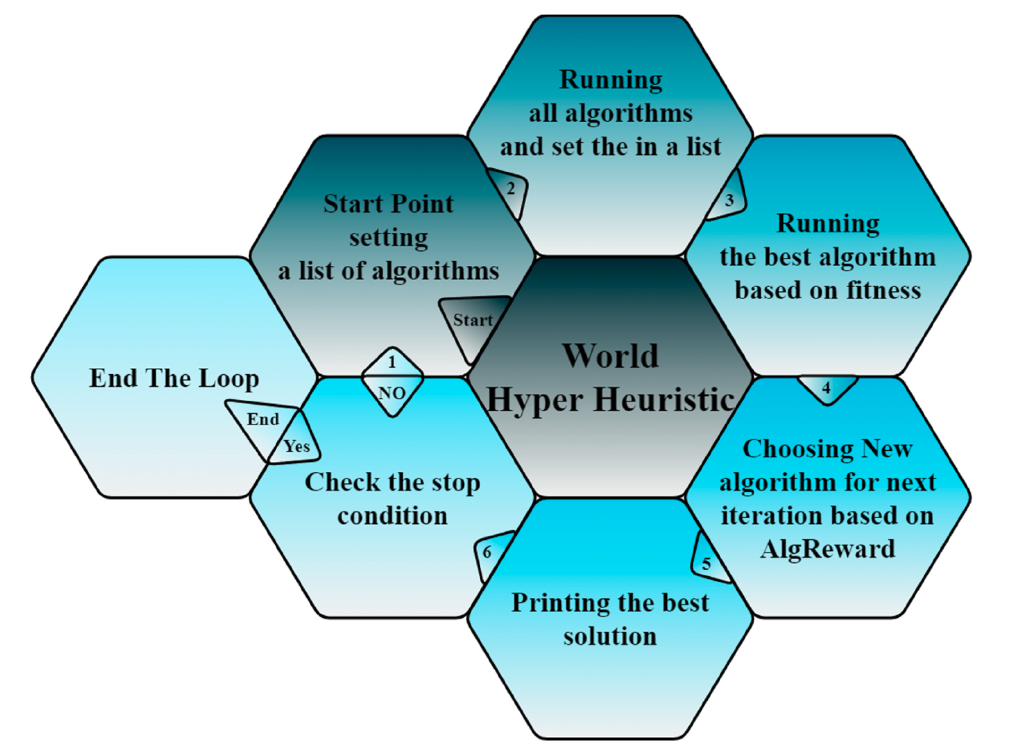
\includegraphics[width=0.8\textwidth]{basic_whh.png}
	\caption{Базовое устройство World Hyper-Heuristic}
	\label{fig:basic_whh}
\end{figure}

\subsection{Вознаграждение}

На первой итерации все алгоритмы начинают с одинаковой случайно сгенерированной популяции решений, и каждая метаэвристика находит свое оптимальное решение. 

Так, пусть изначально мы сгенерировали популяцию из $m$ начальных решений, и алгоритм $i$ получил оптмальное значение функции потерь $L_i$ тогда авторы вводят массив~(\ref{eq:gpopcost})

\begin{equation}
	\label{eq:gpopcost}
		gpopCostA = \{L_1, L_2, \ldots, L_n\}
\end{equation}, где $n$ - число метаэвристик

А затем получаем награды алгоритмов~(\ref{eq:algreward})

\begin{equation}
	\label{eq:algreward}
		AlgReward = \frac{1}{gpopCostA}
\end{equation}

При помощи этих наград наибольший приоритет в поиске решения на первой итерации получит лучший алгоритм

Далее авторы вводят переменную темпа обучения (learning rate) $RLAlpha$ который будет принимать значения в диапазоне [0, 10]

Изначально $RLAlpha = 0$, затем каждую итерацию он будет изменяться согласно~(\ref{eq:rlalpha})

\begin{equation}
	\label{eq:rlalpha}
		RLAlpha = RLAlpha + \frac{1}{maxIter}
\end{equation}, где $maxIter$ - максимальное число итераций

Этот момент уже кажется странным, потому что такая имплементация не даст $RLAlpha$ первысить 1. 

Как будет видно далее по своей сути $RLAlpha$ вообще сложно назвать темпом обучения, а реальный диапазон значений [0, 1] выбран не случайно.

Далее авторы заявляют, что если результат оптимизации не меняется две итерации подряд, то награда лучшего алгоритма уменьшается как показано в выражении~(\ref{eq:rewardchange})

\begin{equation}
	\label{eq:rewardchange}
		AlgReward_{i} = AlgReward_{i} - \frac{\sum_{j = 1}^{j \neq i} AlgReward_{j}}{n}
\end{equation}

\subsection{Селекция}

На первой итерации на фазе селекции просто выбирается алгоритм с наибольшией наградой $AlgReward$

В последующих итерациях на фазе селекции генерируется случайное число $chN$ от 0 до 1, затем если $chN > RLAlpha$ то выбор следующей метаэвристики происходит равновероятно, в ином случае для выбора используется RouletteWheelSelection, рандомный выбор, при котором вероятность выбора метаэвристики пропорциональна величине $AlgReward$

Теперь становится ясно, что $RLAlpha$ это скорее вероятность исследования (exploration), чем темп обучения. 

Видно, что с каждой итерацией эта вероятность уменьшается, что логично, чем больше итераций прошло, тем мы ближе к оптимальному решению и было бы не так разумно отказываться от него, чем на первых шагах.

\begin{figure}
	\centering
	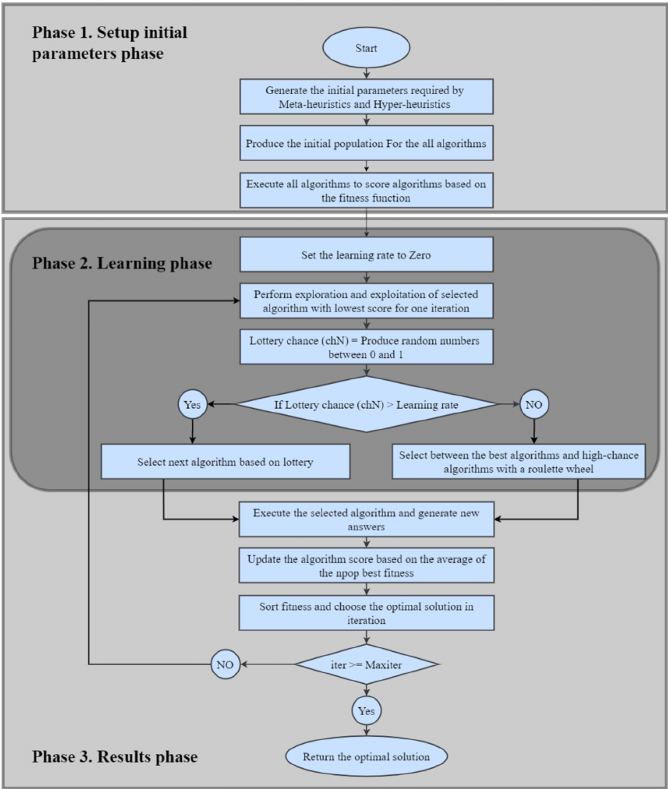
\includegraphics[width=0.8\textwidth]{complex_whh.png}
	\caption{Иллюстрация трех фаз алгоритма}
	\label{fig:complex_whh}
\end{figure}

\section{Анализ результатов приведенных в статье}

Авторы статьи провели несколько экспериментов с целью измерения эффективности WHH по сравнению с классическими метаэвристиками.

Сравнения проводились на дискретных и непрерывных NP-сложных задачах.

Так, например были проведены эксперименты на таких дискретных задачах как проблема коммивояжера на 1000 искусственно сгенерированных городах, координаты которых находятся в диапазоне от 0 до 100.

Авторы также сравненивали свой алгоритм с популярными метаэвристиками на датасете из 10000 реальных городов со всего мира~\cite{RWTCP}.

Третьей дискретной задачей была так называемая $COTEJA$~\cite{COTEJA} (Combinatorial-Optimization-Based Threat Evaluation and Jamming Allocation) - задача представленная в 2019 году, она заключается в поиске сети радаров для обнаружения воздушных судн.

Непрерывные задачи включали в себя поиск глобального минимума 25 функций (см. Таблицу~\ref{table:functions}) 

Также авторы тестировали WHH на реальных проблемах, таких как Welded Beam Design Problem~\cite{weldedbeam} и Speed Reducer Problem~\cite{speedred}

Для дискретных задач авторы использовали набор из 6 метэвристик, их начальные параметры можно увидеть в таблице~\ref{table:initialparamdis}, однако в исходном коде отсутствует реализация Grey Wolf Optimization поэтому я буду считать что авторы отказались от этого алгоритма.

Видно что значения взяты одинаковые для всех алгоритмов, авторы утверждают, что это сделано для того, чтобы все метаэвристики были в равных условиях.

Гиперпараметры специфичные для каждого алгоритма выбраны в соответствии с рекомендованными в соответствующих статьях: Imperialist Competitive Algorithm~\cite{ICA}, Simulated Annealing~\cite{SA}, 	Ant Colony Optimization~\cite{ACO}, Grey Wolf Optimization~\cite{GWO}

Для непрерывных задач начальные параметры также установлены согласно рекоммендациям авторов алгоритмов, значения величины популяции (Population size) и число генераций (Number of generations) для всех алгоритмов одинаковые, всего авторы используют 10 метаэвристик, которые можно увидеть в таблице~\ref{table:initialparamcon}

\section{Анализ исходного кода авторов и воспроизведение полученных результатов}

Заранее стоит сказать, что мною не затронуты возможные ошибки в логике реализации метаэвристик авторами, я сосредоточился на анализе возможных ошибок, допущенных авторами, которые могли бы повлиять на результаты, приведенные в статье.

Код, представленный в статье, вызывает массу вопросов. Отсутствие статической типизации делает его трудным для восприятия. Без явного указания типов данных приходится угадывать, с каким типом данных имеешь дело. Это замедляет процесс анализа и значительно увеличивает вероятность ошибок.

Что касается структуры, то код выглядит перегруженным. Вместо того чтобы делить программу на логичные, самостоятельные блоки, авторы предпочли оставить все в огромных функциях, которые выполняют множество задач одновременно. Это усложняет восприятие, каждый раз приходится разбирать, что именно происходит в функции. Когда код не разделен на логические части, его становится гораздо труднее отлаживать и тестировать.

В частности авторы используют громадное число различных структур данных которые могут даже дублировать друг друга, имена переменных не следуют никакой логике, где-то камелкейс, где-то нижние подчеркивания, одни переменные с большой буквы другие с маленькой, как будто код писали два брата один на клавиатуре другой на мышке.

К примеру в начале основного скрипта авторы вводят частично определенную функцию, однако периодически забывают о ней в процессе и все равно передают зафиксированные параметры.

Вероятно такой подход привел к тому, что сами авторы допустили некоторые критические ошибки.

Так, например в коде дискретного алгоритма WHH в фазе инициализации авторы объявляют 5 используемых метаэвристик, однако запускают только 3, причем награда третьего алгоритма записывается в индекс, в которм уже лежит награда первого, это существенно влияет на всю фазу инициализации -- вместо 5 алгоритмов запускаются только 2, что может сильно влиять на начальные данные для второй фазы. Что еще более забавно, в статье авторы говорят о 6 алгоритмах, в коде объявляют 5 из них, реализованы лишь 3, а записаны результаты только для двух алгоритмов.

Также в коде приложенном авторами полностью отсутствует реализация большинства метаэвристик, который они, как утверждается использовали.

Аналогично, невозможно воспроизвести эксперименты с реальными данными в виду отсутствия реализации взаимодействия я с ними.

Некоторые гиперпараметры переопределяются несколько раз, наример авторы вводят переменную $alpha$ сначала как коэффициент остывания для алгоритма отжига, а затем тут же переопределяют ее как коэффициент $alpha$ в ACO, где он вообще принят целым числом равным 1, что недопустимо для алгоритма отжига, однако авторы избегают ошибок связанных с этим, так как просто понижают температуру не в том месте, где это должно просиходить.

Очень странное также решение авторов в фазе "обучения" они выбирают лучший алгоритм, а затем выбирают случайный алгоритм из Tabu и ICA.

Становися очевидно, что авторами был приложен мало того, что не полный код, который использовался для проведения измерений, этот код содержит множество ошибок и я бы назвал чудом, то что он вообще запускается -- малейшее изменение гиперпараметров, например размерности входных данных приводит к ошибкам и код перестает работать, есть ощущение, что был приложен черновик, а не исходный код к статье.

В связи с этим я переписал код с матлабовских скриптов на питон, а также исправил ошибки (какие нашел) допущенные авторами, добавил статическую типизацию и улушил структуру проекта, для большей читаемости кода, а также реализовал метаэвристики, которых не было в коде авторов.

\section{Моя реализация кода, описанного в статье и сравнение результатов}

Как и описано в статье я использовал для дискретных задач 6 алгоритмов, их начальные параметры.

Для лушчей орагнизации кода я добавил статичную типизацию (насколько это возможно на питоне), а также разделил код на связанные по смыслу классы.

Мною был введен класс Solution, содержащий два поля: Position и Cost -- первое олицетворяет решение задачи, второе значение функции потерь для этого решения.

Авторы использовали похожую структуру данных $empty_individual$, моя реализация сделала код сильно более читаемым, также в классе я объявил стандартный конструктор, использование которого сильно упростило код, а также оператор сравнения, он был необходим для легкой имплементации сортировок.

Каждая метаэвристика также получила свой класс, содержащий методы:

\begin{itemize}
	\item Конструктор - отвечает за инициализацию гиперпараметров метаэвристики
	\item Метод initialize - основной метод, который принимает текущую популяциб и функцию потерь, изменяет популяцию в процессе и возвращает лучшее найденное решение (Solution) в контексте переданной функции потерь
	\item Вспомогательные методы, необходимые для работы алгоритма, например создание соседей, обновление позиций или проверку корректности
\end{itemize}

Такая структура проекта сильно упростила читаемость и воспринимаемость WHH, все метаэвристики мне пришлось реализовывать самому, поэтому насколько качественное это сравнение с реализациями авторов статьи не могу.

Также я полностью переписал основной файл WorldAlg.py под новую структуру проекта, теперь код выглядит последовательным и ясным.

В своей реализации я использовал скрипт run.py для запуска гиперэвристики и построения графиков, далее расскажу о них поподробне. 

Я провел 10 экспериментов с сгенерированной случайной выборкой точек с целочисленными координатами в двумерном пространстве, результаты можно увидеть на графике~\ref{fig:10runs}

Также я построил график с усредненными результами для каждой итерации~\ref{fig:mean_runs} можем легко сравнить его с тем, который авторы приводят в своей статье для этой задачи~\ref{fig:authors_graph}, конечно они вычислительные мощности у них боли существенно больше, поэтому провести 1000 экспериментов я не смог, но и 10 достаточно, чтобы заметить схожесть вида графиков, однако алгоритм переписанный мной получил ощутимо лучшие результаты.

\section{Заключение}

В заключение хочется сказать, что несмотря на ужасный код, приложенный авторами под видом исходного, сам алгоритм при должном подходе код становится понятным и масштабируемым, в дальшейшем можно произвести любое число модификаций моей реализации и добиться еще более впечатляющих результатов.

В дальнейшем я не планирую забрасывать существующий проект и планирую развивать его дальше, в близжайших планах реализовать свою версию для непрерывного алгоритма. Также я хочу улучшить структуру кода, добавить больше абстракций, расширяя просторы для расширения функционала. Не помешает также создать удобный интерфейс (хотя бы скрипт) для тюнинга параметров и, например загрузки пользовательской задачи оптимизации.

Как видно, современные ученые сильно продвинулись в области поиска субоптимальных решений NP-сложных задач, что не может не радовать. Надеюсь авторы не забросят свои наработки, и продолжат развивать эту идею, например можно внедрить реальное машинное обучение, а еще надеюсь, что они все-таки опубликуют оригинальный код.

\begin{figure}[ht]
	\centering
	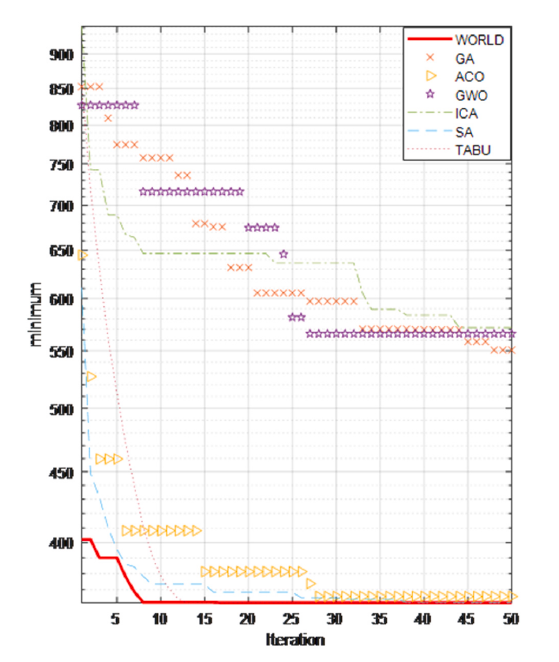
\includegraphics[width=0.8\textwidth]{authors_graph.png}
	\caption{График результатов, полученных авторами статьи}
	\label{fig:authors_graph}
\end{figure}

\begin{figure}[ht]
	\centering
	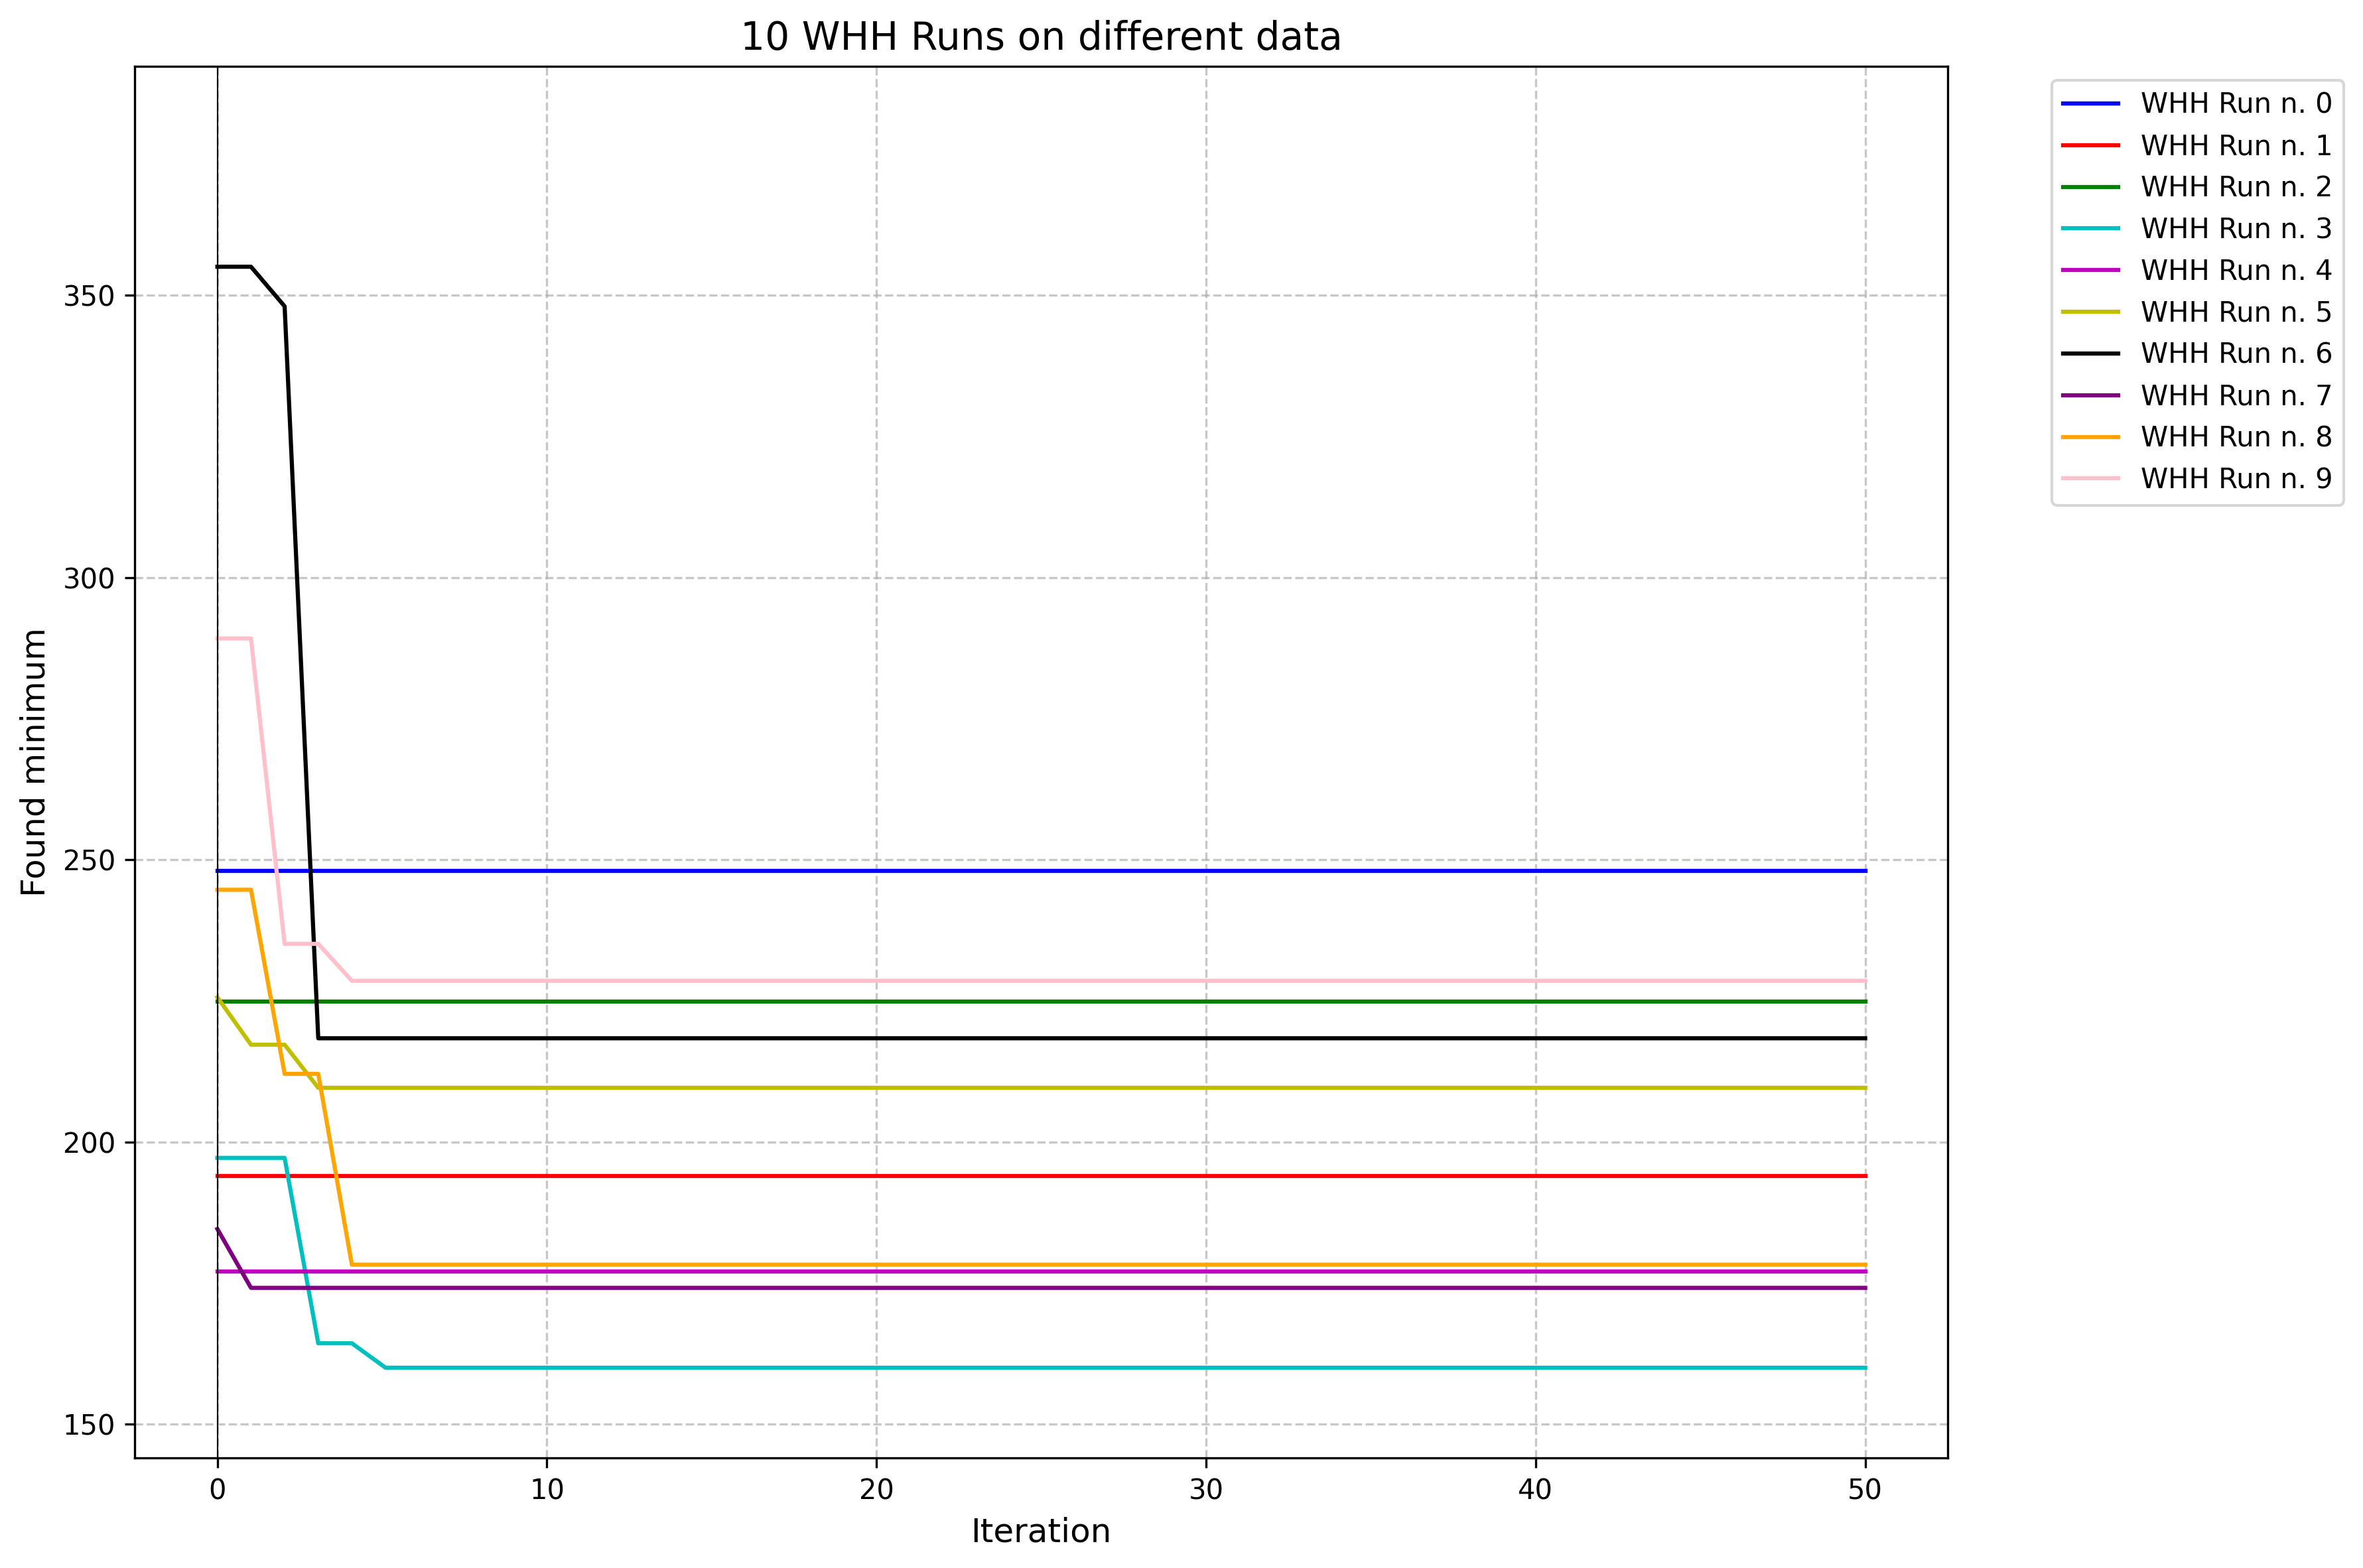
\includegraphics[width=0.8\textwidth]{10Runs.png}
	\caption{График минимального значения, найденного алгоритмом на каждой итерации}
	\label{fig:10runs}
\end{figure}

\begin{figure}[ht]
	\centering
	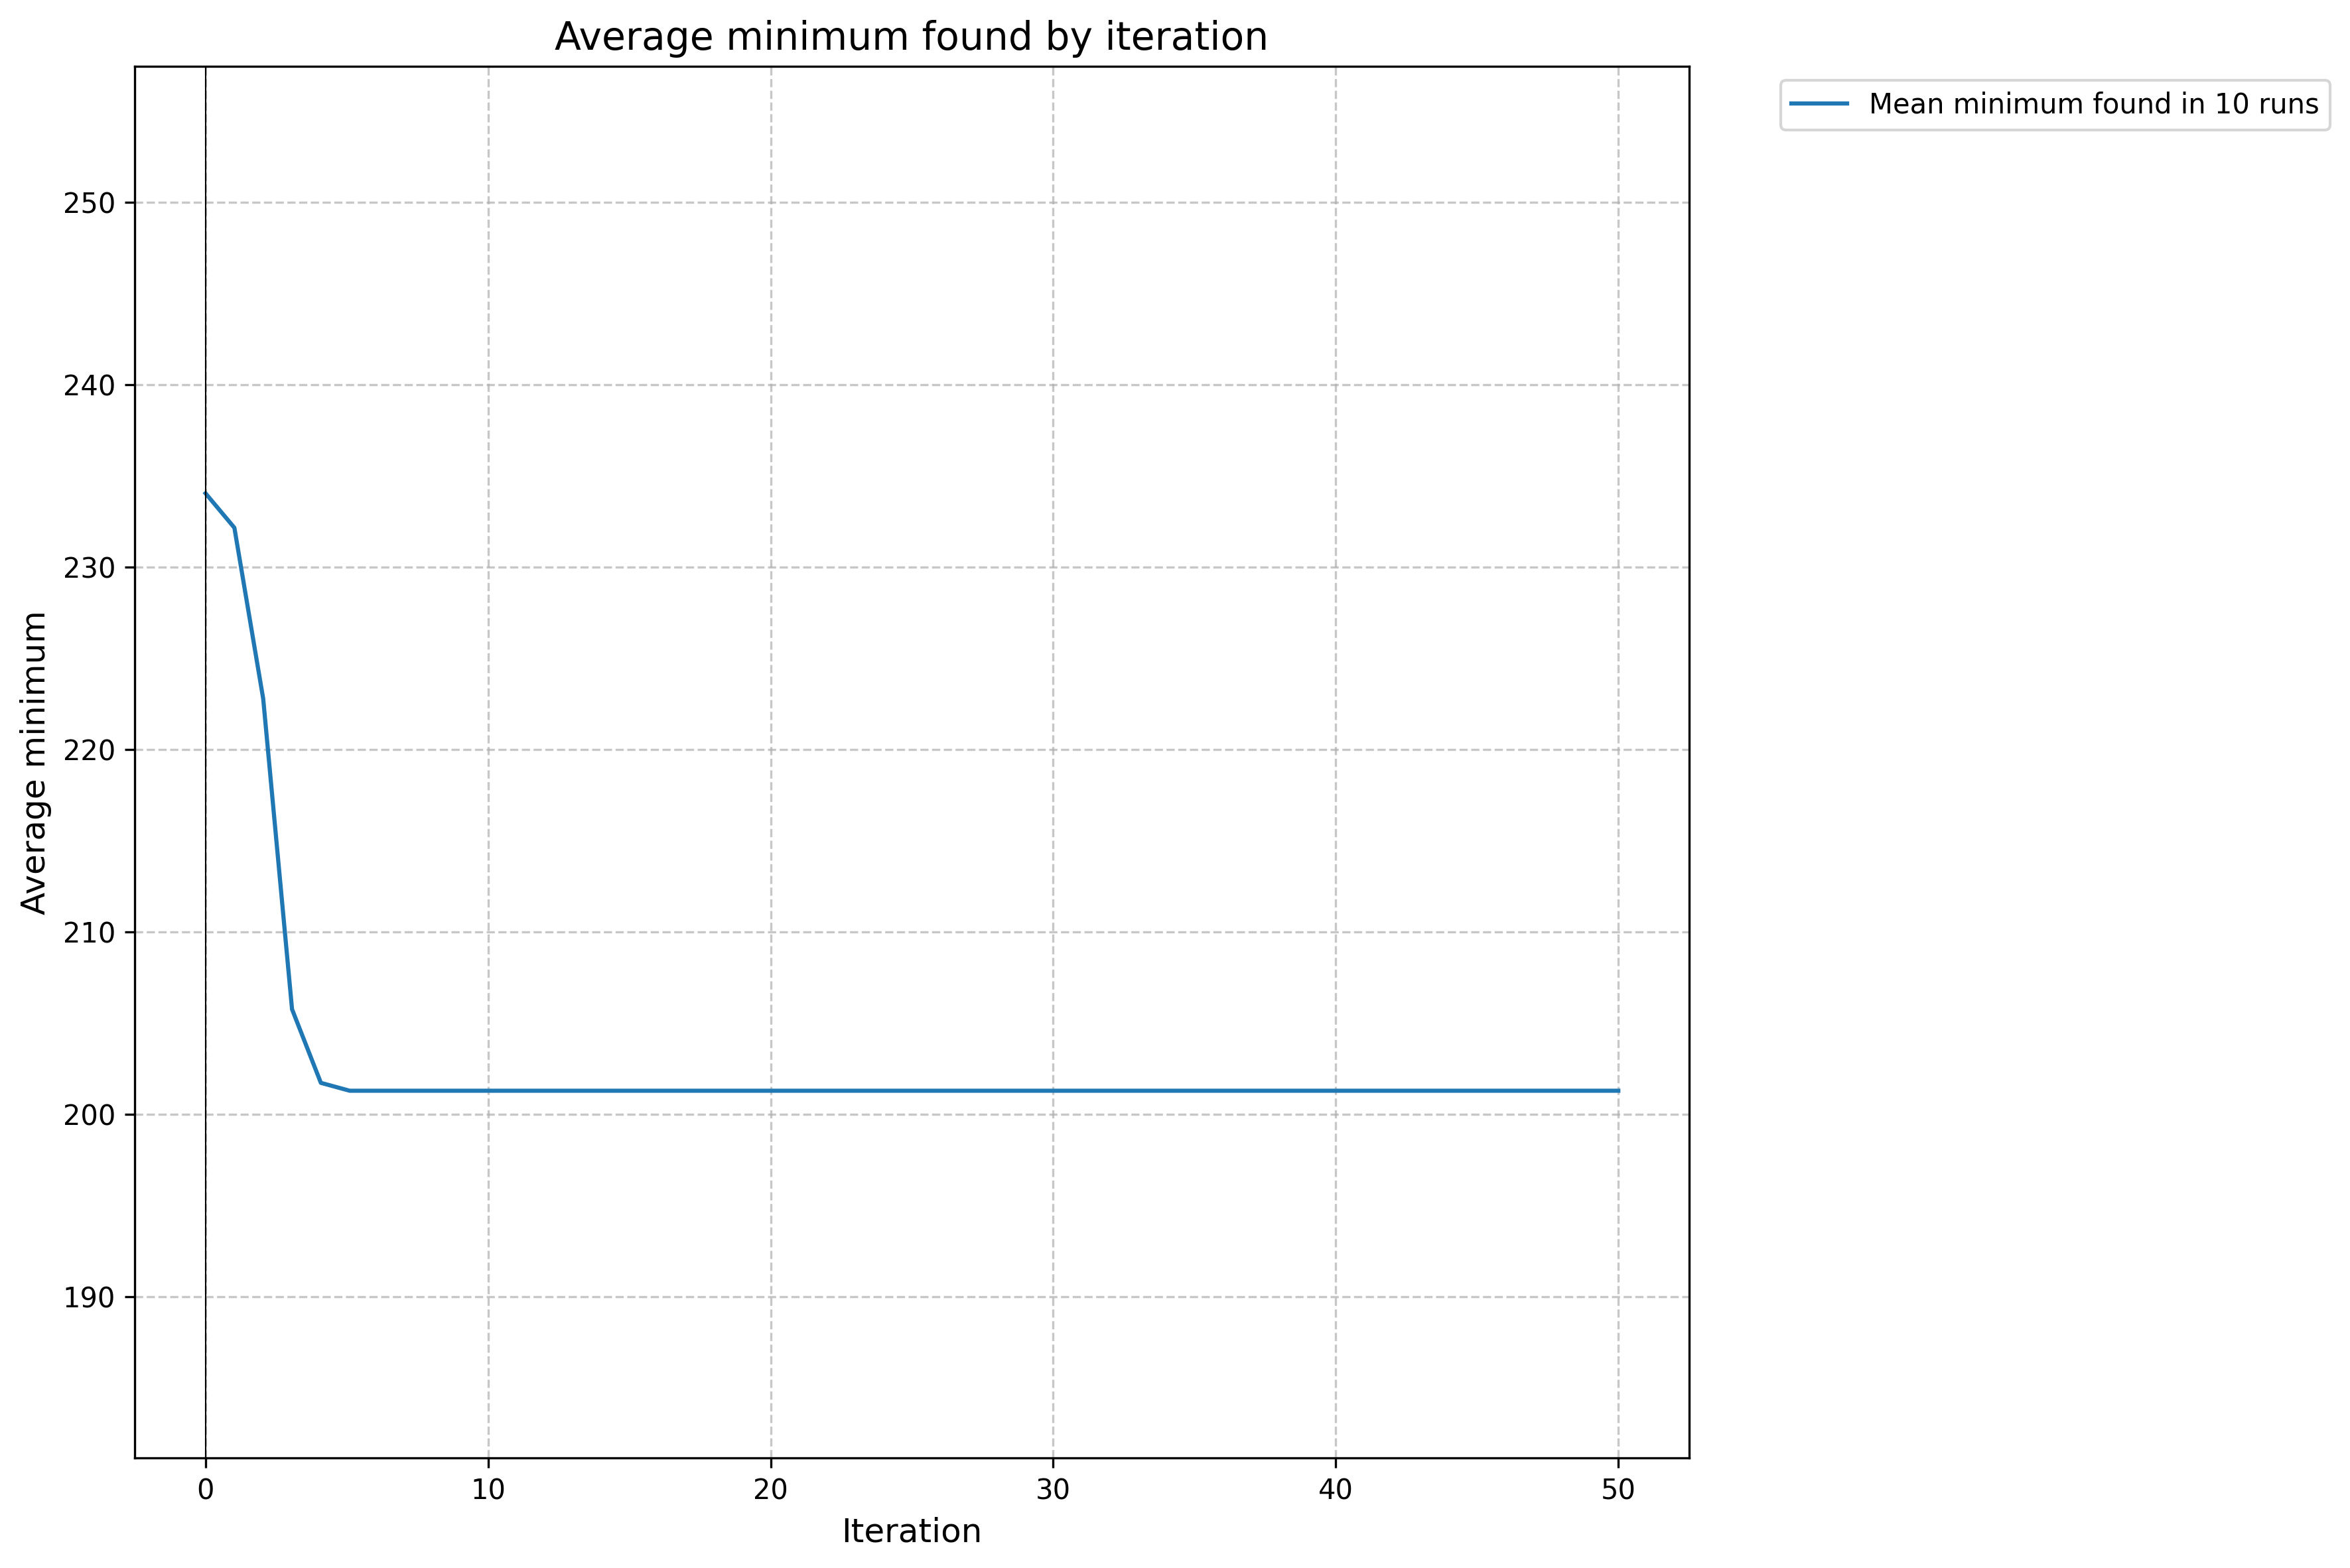
\includegraphics[width=0.8\textwidth]{MeanRuns.png}
	\caption{График среднего минимального значения, найденного алгоритмом на каждой итерации}
	\label{fig:mean_runs}
\end{figure}

\begin{table}[ht]
	\caption{Функции, на которых проводились эксперименты авторами статьи. В столбце $Fmin$ указан глобальный минимум}
	\label{table:functions}
	\footnotesize
	\centering
	\begin{tabular}{lcr}
		\toprule
		Название функции &  Формулы &  Fmin \\
		\midrule
		Ackley & $f(x) = f(x_1, \ldots, x_n) = - a \cdot \exp\left(-b\sqrt{\frac{1}{n}\sum_{i = 1}^{n}x_{i}^{2}}\right) - \exp\left(\frac{1}{n}\sum_{i=1}^{n} \cos(c x_i)\right) + a + \exp(1)$ & 0\\
		Brown & $f(x) = \sum_{i = 1}^{n - 1} {(x_i)}^{x_{i+1}^{2} + 1} + {(x_{i+1}^{2})}^{x_{i}^{2} + 1}$ & 0\\
		Exponential & $f(x) = - \exp\left(-0.5 \sum_{i = 1}^{n} x_i^2\right)$ & -1\\
		Griewank & $f(x) = 1 + \sum_{i = 1}^{n} \frac{x_i^2}{4000} - \prod_{i = 1}^{n} \cos\left(\frac{x_i}{\sqrt{i}}\right)$ & 0\\
		Periodic & $f(x) = 1 + \sum_{i = 1}^{n} \sin^2 (x_i) - 0.1 \exp\left(\sum_{i = 1}^{n} x_i^2\right)$ & 0.9\\
		Powell Sum & $f(x) = \sum_{i = 1}^{n} {|x_i|}^{i + 1}$ & 0\\
		Qing & $f(x) = \sum_{i = 1}^{n} (x_i^2 - i)^2$ & 0\\
		Quartic & $f(x) = \sum_{i = 1}^{n} ix_i^4 + random[0, 1)$ & 0\\
		Rastrigin & $f(x) = 10n + \sum_{i = 1}^{n} (x_i^2 - 10 \cos(2\pi x_i))$ & 0\\
		Ridge & $f(x) = x_1 + d \left(\sum_{i = 2}^{n} x_i^2\right)^{\alpha}$ & -10\\
		Rosenbrock & $f(x) = \sum_{i = 1}^{n-1} b(x_{i+1} - x_i^2)^2 + (a - x_i)^2$ & 0\\
		Salomon & $f(x) = 1 - \cos \left(2\pi \sqrt{\sum_{i = 1}^{n} x_i^2}\right) + 0.1 \sqrt{\sum_{i = 1}^{n} x_i^2}$ & 0\\
		Schwefel 2.20 & $f(x) = \sum_{i = 1}^{n} |x_i|$ & 0\\
		Schwefel 2.21 & $f(x) = \max |x_i|$ & 0\\
		Schwefel 2.22 & $f(x) = \sum_{i = 1}^{n} |x_i| + \prod_{i = 1}^{n} |x_i|$ & 0\\
		Schwefel 2.23 & $f(x) = \sum_{i = 1}^{n} x_i^{10}$ & 0\\
		shubert3 & $f(x) = \sum_{i = 1}^{n} \sum_{j = 1}^{5} j \sin ((j + 1)x_i + j)$ & -101\\
		Sphere & $f(x) = \sum_{i = 1}^{n} x_i^2$ & 0\\
		Styblinski-Tank & $f(x) = \frac{1}{2} \sum_{i = 1}^{n} x_i^4 - 16x_i^2 + 5x_i$ & -200\\
		Sum Squares & $f(x) = \sum_{i = 1}^{n} ix_i^2$ & 0\\
		Xin-She Yang & $f(x) = \sum_{i = 1}^{n} \in_i |x_i|^i$ & 0\\
		Xin-She Yang N. 2 & $f(x) = \left(\sum_{i = 1}^{n} |x_i|\right)\exp\left(\sum_{i = 1}^{n}\sin(x_i^2)\right)$ & 0\\
		Xin-She Yang N. 3 & $f(x) = \exp\left(-\sum_{i=1}^{n} \left(\frac{x_i}{\beta}\right)^{2m} - 2\exp\left(-\sum_{i = 1}^{n} x_i^2\right)\prod_{i = 1}^{n} \cos^2 (x_i)\right)$ & 0\\
		Xin-She Yang N. 4 & $f(x) = \left(\sum_{i = 1}^{n} \sin^2(x_i) - \exp\left(-\sum_{i = 1}^{n} x_i^2\right)\right) \exp\left(-\sum_{i = 1}^{n} \sin^2 \sqrt{|x_i|}\right)$ & -1\\
		Zakharov & $f(x) = \sum_{i =1 }^{n} x_i^2 + \left(0.5 \sum_{i = 1}^{n} i x_i\right)^2 + \left(0.5 \sum_{i =1 }^{n} i x_i\right)^4$ & 0\\
		% \midrule
		\bottomrule
	\end{tabular}
\end{table}

\begin{table}[ht]
	\caption{Начальные параметры метаэвристик для дискретных задач}
	\label{table:initialparamdis}
	\footnotesize
	\centering
	\begin{tabular}{lp{0.25\linewidth}p{0.25\linewidth}}
		\toprule
		Алгоритм &  Параметры &  Значения \\
		\midrule
		Ant Colony Optimization (ACO) & Population Size \newline
										Number of generations \newline
										Conversion ratio fitness & 50\newline
																   100\newline
																   100\\
		Genetic Algorithm (GA) & Population Size \newline
								 Number of generations of 10,000 cities \newline
								 Number of generations for others & 50 \newline
								 								    1000 \newline
																	100\\
		Grey Wolf Optimization (GWO) & Control Parameter \newline
								 	   Number of generations of 10,000 cities \newline
								 	   Number of generations for others \newline
									   Number of particles & [0, 2] \newline
															 1000 \newline
															 100 \newline
															 50\\
		Imperialist Competitive Algorithm (ICA) & Number of countries \newline
												  Number of generations of 10,000 cities \newline
												  Number of generations for other \newline
												  Number of nimp & 50 \newline
												  				   1000 \newline
																   100 \newline
																   10\\
		Simulated Annealing (SA) & Population Size \newline
								   Number of generations of 10,000 cities \newline
								   Number of generations for other \newline
								   Number of neigbors & 50 \newline
												  		1000 \newline
														100 \newline
														10\\
		Tabu (Taboo) & Population Size \newline
					   Number of generations of 10,000 cities \newline
					   Number of generations for other & 50 \newline
														 1000 \newline
														 100 \\
		\bottomrule
	\end{tabular}
\end{table}

\begin{table}[ht]
	\caption{Начальные параметры метаэвристик для непрерывных задач}
	\label{table:initialparamcon}
	\footnotesize
	\centering
	\begin{tabular}{lp{0.25\linewidth}p{0.25\linewidth}}
		\toprule
		Алгоритм &  Параметры &  Значения \\
		\midrule
		Adaptive differential evolution algorithm (ADEA) & Population Size \newline
														   Number of generations  & 50\newline
														   						    1000\\
		Artificial bee colony algorithm  (ABC) & Population Size \newline
								 N				 Number of generations & 50\newline
								 										 1000\\
		Biogeography Optimization (BO) & Alpha \newline
								 	   Number of generations \newline
								 	   Keep Rate & 0.9 \newline
												   1000 \newline
												   0.4\\
		Differential Evolution (DE) & Beta min \newline
									  Beta max \newline
									  PCR \newline
									  Number of generations & 0.2 \newline
												  			  0.8 \newline
															  0.2 \newline
															  1000\\
		Firefly Algorithm (FA) & Gamma \newline
								 Beta \newline
								 Number of generations & 1 \newline
												  		 2 \newline
														 1000\\
		Genetic Algorithm  (GA) & Population Size \newline
					   			  Number of generations \newline
					   			  Gamma & 50 \newline
										  1000 \newline
										  0.4\\
		Harmony Search (HS) & Number of nimp \newline
								  Neigboring value rate \newline
								  Discrete set and fret \newline
								  Width \newline
								  Number of generations & 10 \newline
								 		  				  0.3 \newline
								 		  				  17700,1 \newline
														  1000\\
		Improved Invasive Weed Optimization (IWO) & Exponent \newline
													Sigma initial \newline
													Sigma final \newline
													Number of generations & 2 \newline
																			0.5 \newline
																			0.001 \newline
																			1000\\
		Particle Swarm Optimization (PSO) & Inertia coefficient \newline
											Cognitive \& social coeff \newline
											Number of generations \newline
											Search agents & 0.75 \newline
															[1.8, 2] \newline
															1000 \newline
															100\\
		Self-adaptive Differential Evolution Algorithm (SADE) & Population size \newline
																Number of generations & 50 \newline
																						1000\\
		Shuffled Frog-Leaping Algorithm (SFLA) & Memeplex \newline
												 Alpha \newline
												 Beta \newline
												 Number of generations & 10 \newline
												 						 3 \newline
																		 5 \newline
																		 1000\\
		Simulated Annealing (SA) & Alpha \newline
								   Mu \newline
								   Number of generations & 0.99 \newline
								   						   0.5 \newline
														   1000\\
		Single objective real-parameter optimization (jSO) & Population Size \newline
															 Number of generations & 50 \newline
															 						 1000\\
		Teaching-Learning Optimization Algorithm (TLBO) & Population Size \newline
														  Number of generations & 50 \newline
														  						  1000\\
		\bottomrule
	\end{tabular}
\end{table}

\newpage 
\printbibliography[heading=bibintoc] 

% \begin{thebibliography}{0}
% 	\bibitem{chirkova18}\hypertarget{chirkova18}{}
% 	\href{https://arxiv.org/abs/1810.10927}
% 	{Nadezhda Chirkova, Ekaterina Lobacheva, Dmitry Vetrov. Bayesian Compression for Natural Language Processing. In EMNLP 2018.}
% \end{thebibliography}
	
\newpage

\end{document}
